De verschillende $\alpha$ waarden hebben een invloed op de ligging van de eigenwaarden alsook het conditiegetal $\kappa(A)$ van A. Voor $\alpha = 1$ is het conditiegetal $\kappa(A) = 9.4108*10^3$, voor $\alpha = 5$ is $\kappa(A) = 46.6201$, voor $\alpha = 10$ is $\kappa = 13.3134$ en tot slot voor $\alpha = 100$ is $\kappa(A) = 1.5601$.\\[12pt]

Wanneer we nu de eigenwaarden gaan bekijken zien we dat de eigenwaarden bij \ref{alpha 1} het meest verspreid liggen en het meest naar het centrum, hoe hoger de $\alpha$ waarde hoe verder de meeste eigenwaarden zich naar de rand van de eenheidscirkel begeven en dichter bij elkaar komen te liggen. Dit komt ook overeen met de eigenschap:\\[12pt]
 $\|r_{n}\| \leq inf\|p(A)\| \leq \kappa_{2}(V) inf (max |p(\lambda)|\|r_{0}\|),\forall p\in P_{n}, \forall\lambda\in \sigma(A)$.\\[12pt]
 Deze stelt immers dat snelle convergentie bereikt wordt voor eigenwaarde van A die geclusterd zitten, weg van de oorsprong en met A gelijkend op een normaal matrix ($A*A^{*} = A^{*}*A$).

\begin{figure}[H]
  \centering
  \subfloat[alpha 1]{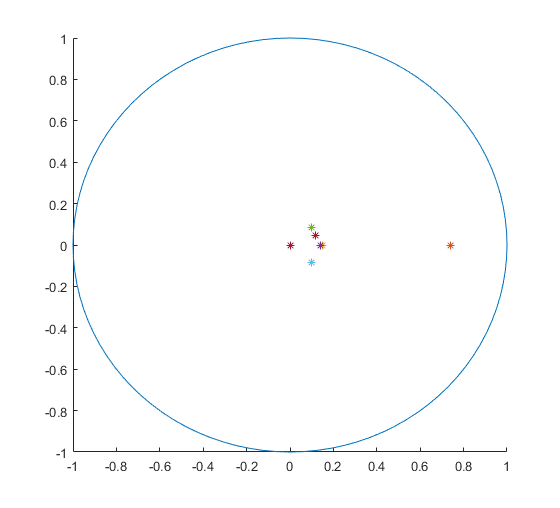
\includegraphics[width=0.5\textwidth]{Tekeningen/GMRES_alpha1_eigenv}\label{alpha 1}}
  \hfill
  \subfloat[alpha 5]{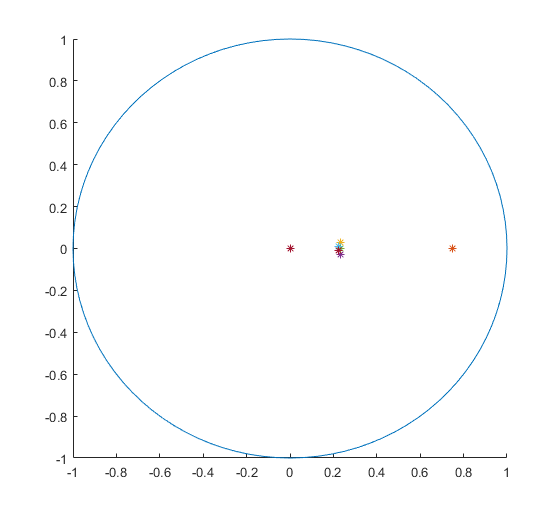
\includegraphics[width=0.5\textwidth]{Tekeningen/GMRES_alpha5_eigenv}\label{alpha 5}}
  \caption{Links eigenwaarden voor $\alpha = 1$, rechts voor $\alpha = 5$}
\end{figure}

\begin{figure}[H]
  \centering
  \subfloat[alpha 10]{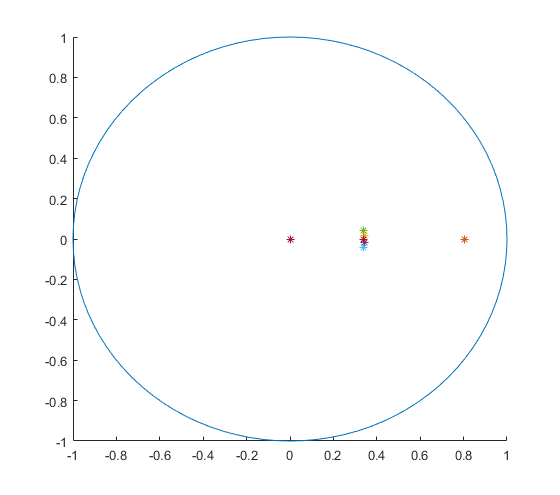
\includegraphics[width=0.5\textwidth]{Tekeningen/GMRES_alpha10_eigenv}\label{alpha 10}}
  \hfill
  \subfloat[alpha 100]{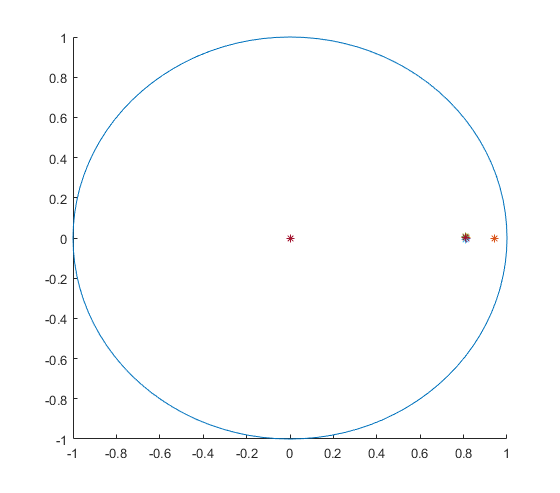
\includegraphics[width=0.5\textwidth]{Tekeningen/GMRES_alpha100_eigenv}\label{alpha 100}}
  \caption{Links eigenwaarden voor $\alpha = 10$, rechts voor $\alpha = 100$}
\end{figure}

\begin{figure}[H]
  \centering
  \subfloat[fout op $\|r_{n}\|$]{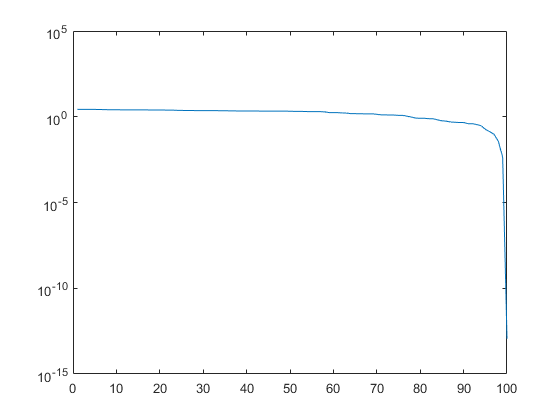
\includegraphics[width=0.5\textwidth]{Tekeningen/GMRES_alpha1_r}\label{r_1}}
  \hfill
  \subfloat[fout op exacte oplossing]{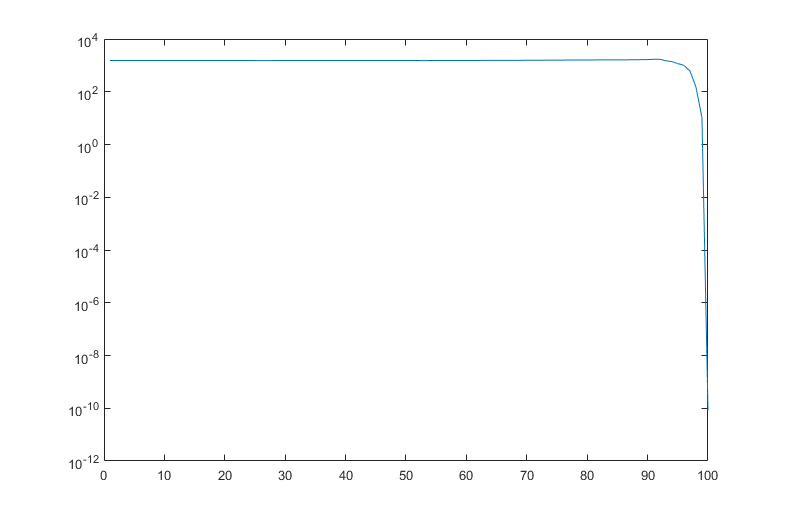
\includegraphics[width=0.5\textwidth]{Tekeningen/GMRES_alpha1_x-y}\label{x-y_1}}
  \caption{Resp. fouten voor $\alpha = 1$.}
\end{figure}

\begin{figure}[H]
  \centering
  \subfloat[fout op $\|r_{n}\|$]{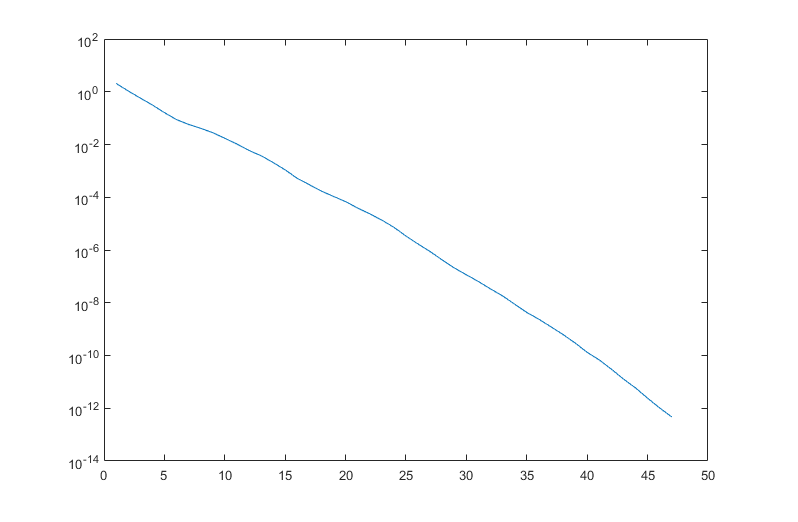
\includegraphics[width=0.5\textwidth]{Tekeningen/GMRES_alpha5_r}\label{r_5}}
  \hfill
  \subfloat[fout op exacte oplossing]{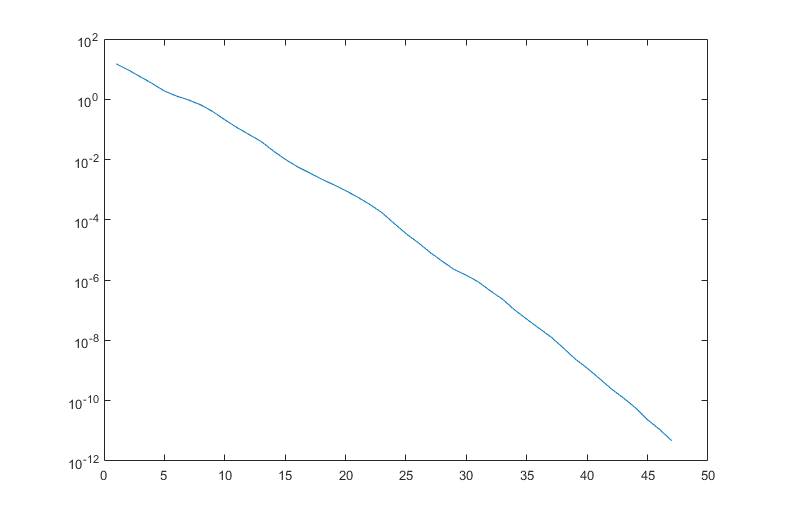
\includegraphics[width=0.5\textwidth]{Tekeningen/GMRES_alpha5_x-y}\label{x-y_5}}
  \caption{Resp. fouten voor $\alpha = 5$.}
\end{figure}

\begin{figure}[!tbp]
  \centering
  \subfloat[fout op $\|r_{n}\|$]{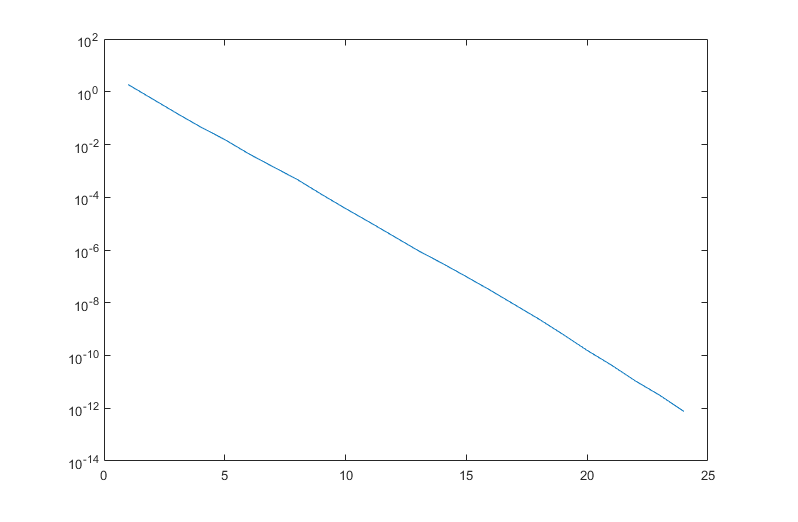
\includegraphics[width=0.5\textwidth]{Tekeningen/GMRES_alpha10_r}\label{r_10}}
  \hfill
  \subfloat[fout op exacte oplossing]{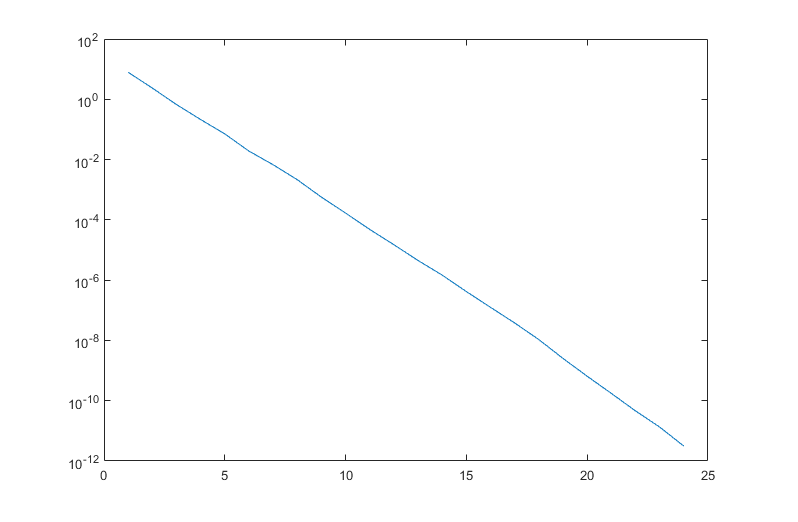
\includegraphics[width=0.5\textwidth]{Tekeningen/GMRES_alpha10_x-y}\label{x-y_10}}
  \caption{Resp. fouten voor $\alpha = 10$.}
\end{figure}

\begin{figure}[!tbp]
  \centering
  \subfloat[fout op $\|r_{n}\|$]{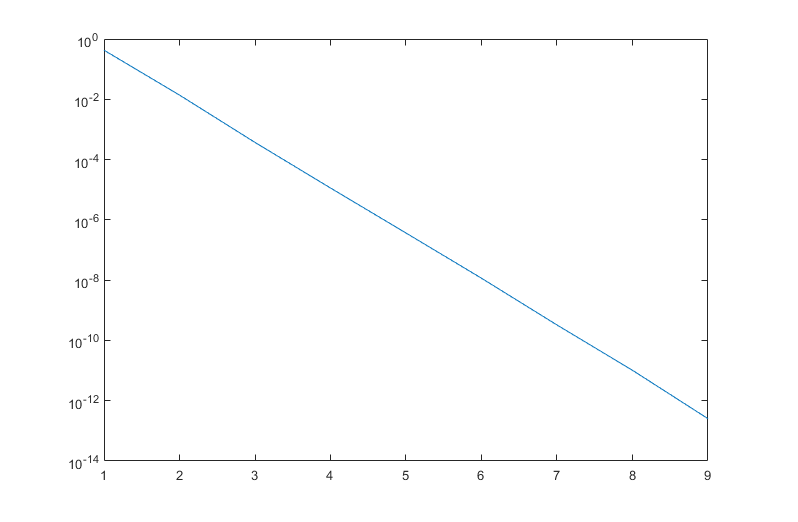
\includegraphics[width=0.5\textwidth]{Tekeningen/GMRES_alpha100_r}\label{r_100}}
  \hfill
  \subfloat[fout op exacte oplossing]{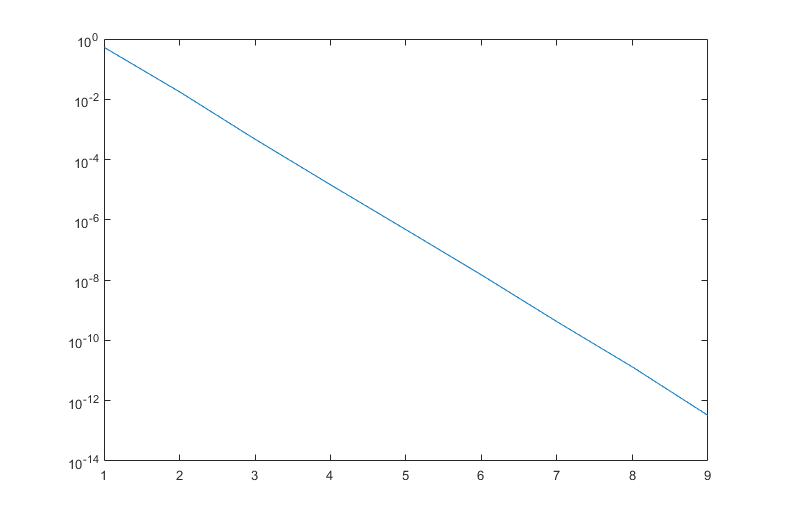
\includegraphics[width=0.5\textwidth]{Tekeningen/GMRES_alpha100_x-y}\label{x-y_100}}
  \caption{Resp. fouten voor $\alpha = 100$.}
\end{figure}


